\documentclass[czech]{article}
\usepackage[T1]{fontenc}
\usepackage[utf8]{inputenc}
\usepackage[a4paper]{geometry}
\geometry{verbose,tmargin=2cm,bmargin=2cm,lmargin=1.5cm,rmargin=1.5cm}
\usepackage{fancyhdr}
\pagestyle{fancy}
\usepackage{babel}
\usepackage{array}
\usepackage{float}
\usepackage{fancybox}
\usepackage{calc}
\usepackage{graphicx}
\usepackage[unicode=true,
 bookmarks=true,bookmarksnumbered=false,bookmarksopen=false,
 breaklinks=false,pdfborder={0 0 0},backref=false,colorlinks=false]
 {hyperref}
\hypersetup{pdftitle={Konfigurace programu},
 pdfauthor={xkovl007},
 pdfsubject={Konfigurace programu},
 pdfkeywords={xml,schema,json,html,LaTeX}}

\makeatletter

\providecommand{\tabularnewline}{\\}

\makeatother

\begin{document}

\title{Nastavení programu}


\author{Lukáš Kovář (xkovl007)}


\date{19.4.2017}
\maketitle
\begin{abstract}
Tato práce pojednává o tvorbě konfigurace ve formátu XML, schématu
XML, XML transformátoru do JSON, html dokumentace a \LaTeX dokumentace
do předmětu ``Značkovací jazyky''
\end{abstract}
\newpage{}

\tableofcontents{}

\listoffigures


\listoftables


\newpage{}


\section{Úvod}

Tento dokument pojednává o semestrálním projektu pro předmět \textquotedbl{}Značkovací
jazyky\textquotedbl{}, jehož tématem bylo navrhnout nastavení/konfiguraci
(smyšlené) aplikace.

Semestrální projekt obsahuje následující soubory:

\begin{center}
\begin{table}[H]
\begin{centering}
\begin{tabular}{|c|>{\centering}p{10cm}|}
\hline 
\textbf{Název souboru} & \textbf{Popis souboru}\tabularnewline
\hline 
\hline 
\textbf{popis.html} & HTML soubor s popisem tohoto projektu\tabularnewline
\hline 
\textbf{nastaveni.xml} & XML soubor obsahující konfiguraci smyšleného počítačového programu\tabularnewline
\hline 
\textbf{nastaveni.xsd} & XML schéma výše uvedeného XML souboru\tabularnewline
\hline 
\textbf{xml\_to\_json.xsl} & XML transformační dokument pro převod výše uvedeného XML souboru do
JSON souboru\tabularnewline
\hline 
\textbf{nastaveni.json} & JSON soubor vygenerovaný pomocí transformačního dokumentu XSL\tabularnewline
\hline 
\textbf{nepojmenovany.png} & Snímek obrazovky doposud nepojmenovaného programu\tabularnewline
\hline 
\textbf{popis.tex} & \LaTeX soubor s popisem projektu\tabularnewline
\hline 
\textbf{popis.pdf} & PDF soubor s popisem tohoto projektu vygenerovaný pomocí pdflatex
ze souboru ,,popis.tex``\tabularnewline
\hline 
\textbf{zadani.txt} & Zadání tohoto projektu zadané cvičícím/přednášejícím\tabularnewline
\hline 
\textbf{README.md} & Soubor obsahující jednoduchý popis repozitáře github\tabularnewline
\hline 
\textbf{LICENSE.md} & Soubor obsahující text permisivní licence MIT (pro github)\tabularnewline
\hline 
\end{tabular}
\par\end{centering}

\caption{Soubory v repozitáři}
\end{table}

\par\end{center}


\section{Metodika}

Nejprve byl navržen XML soubor, ze kterého bylo následně derivováno
XML schéma a testován transformační dokument pro převod XML souboru
do JSON souboru.


\subsection{Použité nástroje}

Pro vytvoření souborů bylo využito většího množství programů a nástrojů,
přičemž jeden program dokonce vznikl samostatně pouze pro zjednodušení
práce s tímto projektem.

\begin{table}[H]
\begin{centering}
\begin{tabular}{|c|>{\centering}p{10cm}|}
\hline 
\textbf{Název nástroje} & \textbf{Důvod využití}\tabularnewline
\hline 
\hline 
\textbf{NetBeans} & Kontrola syntaxe, transformace XML, pretty printing\tabularnewline
\hline 
\textbf{Doposud nepojmenovaný program} & Kontrola syntaxe, kontrola správnosti JSON výstupu, podpora při tvorbě
XML schématu, ověření XML schématu, kontrola html, transformace, pretty
printing\tabularnewline
\hline 
\textbf{Kate} & Kontrola syntaxe, html, \LaTeX{}\tabularnewline
\hline 
\textbf{Bluefish} & ditto\tabularnewline
\hline 
\textbf{wc (word counter)} & Program pro počítání znaků/řádek na Unixových operačních systémech\tabularnewline
\hline 
\textbf{pdflatex} & Generování výstupního PDF souboru z vstupního \LaTeX{} souboru\tabularnewline
\hline 
\end{tabular}
\par\end{centering}

\caption{Využité programy}
\end{table}


\begin{figure}[H]
\begin{centering}
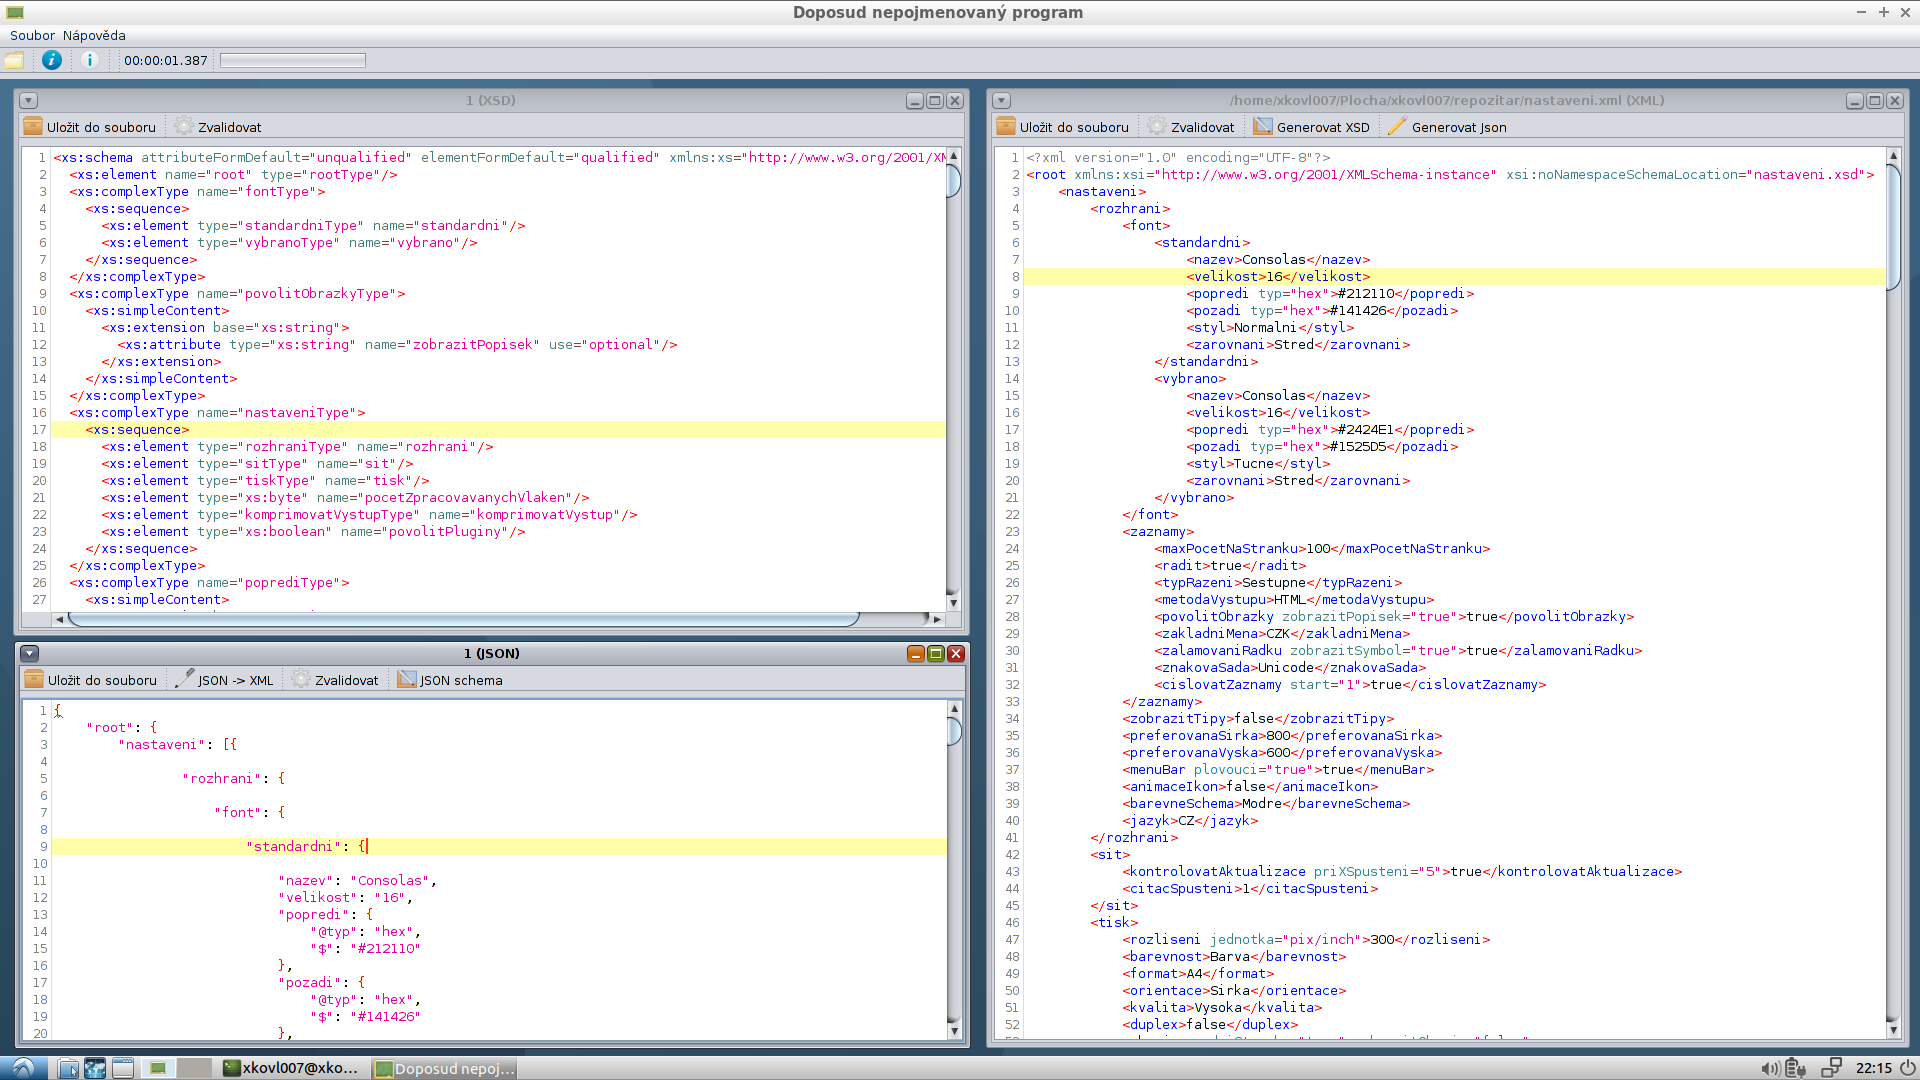
\includegraphics[scale=0.35]{nepojmenovany}
\par\end{centering}

\caption{Snímek obrazovky doposud nepojmenovaného programu}
\end{figure}



\section{Popis elementů a atributů}

Zamýšlená konfigurace aplikace se zaměřuje na tisk, velikost oken,
síť a určitý druh záznamů.

Zde je uveden výčet některých elementů a atributů, které se vyskytují
v XML souboru, jeho schématu a vygenerovaném JSON souboru.

XML obsahuje jeden kořenový element \textquotedbl{}\textbf{root}\textquotedbl{},
do kterého je vnořeno celkem 5 konfigurací (ukázkových záznamů), jak
je požadováno v zadání. Do samotné konfigurace jsou vnořeny další
elementy, některé elementy mají ještě zadány atributy.

Element \textquotedbl{}\textbf{rozhrani}\textquotedbl{}, který je
vnořen do elementu \textquotedbl{}\textbf{nastaveni}\textquotedbl{},
představuje konfiguraci (hypotetického) grafického rozhraní, které
je zobrazeno koncovému uživateli.

V elementu \textquotedbl{}\textbf{rozhrani}\textquotedbl{} se nachází
element \textquotedbl{}\textbf{font}\textquotedbl{}, který nastavuje
vzhled písma (\textquotedbl{}\textbf{standardni}\textquotedbl{} a
\textquotedbl{}\textbf{vybrano}\textquotedbl{}), tedy dvě konfigurace,
pokud je text nevybrán a vybrán; u sub-elementu \textquotedbl{}\textbf{popredi}\textquotedbl{}
a \textquotedbl{}\textbf{pozadi}\textquotedbl{} je atributem uvedeno,
v jakém formátu je zadaná hodnota barvy uvedena (příklad: hex: \#161616
nebo dec: 100,50,100).

Dalším sub-elementem v \textquotedbl{}\textbf{rozhrani}\textquotedbl{}
je i element \textquotedbl{}\textbf{zaznamy}\textquotedbl{}, který
může představovat seznam záznamů, které jsou uživateli představovány.

\textquotedbl{}\textbf{zobrazitTipy}\textquotedbl{} nastavuje, zda
se uživateli po startu budou zobrazovat (nepříjemné) tipy programu.

\textquotedbl{}\textbf{preferovanaSirka}\textquotedbl{} a \textquotedbl{}\textbf{preferovanaVyska}\textquotedbl{}
určují, jak velké bude okno aplikace při startu.

\textquotedbl{}\textbf{menuBar}\textquotedbl{} označuje lištu nástrojů
a zda má tato lišta být zobrazena.

\textquotedbl{}\textbf{nastaveni}\textquotedbl{} dále obsahuje element
\textquotedbl{}\textbf{sit}\textquotedbl{}, který určuje, jakým způsobem
bude program pracovat se sítí; v tomto případě je k dispozici sub-element,
který určuje, zda-li se budou kontrolovat aktualizace a atribut určuje,
jak často tomu tak bude (kolikáté spuštění aplikace), přičemž čítač
spuštění aplikace je uveden v dalším elementu, v tomto případě je
tedy při každém otevření aplikace soubor s nastavením nutné pokaždé
aktualizovat, což v některých případech nemusí být žádoucí, v takovém
případě je možné čítač odstranit a nechat pouze boolean hodnotu, jestli
má aplikace být aktualizována při každém spuštění. 

Element \textquotedbl{}\textbf{tisk}\textquotedbl{} určuje nastavení
tiskárny při posílání výstupu na tiskárnu.

\textquotedbl{}\textbf{rozliseni}\textquotedbl{} je uváděno včetně
atributu, který určuje jednotku.

Atribut \textquotedbl{}\textbf{uvodniStranka}\textquotedbl{} u elementu
\textquotedbl{}\textbf{okraje}\textquotedbl{} určuje, zda-li se i
úvodní stránka bude řídit okraji zbytku dokumentu. V opačném případě
by na tuto úvodní stránku byl vytištěn pouze název dokumentu.

Atribut \textquotedbl{}\textbf{zobrazitOkraje}\textquotedbl{} zapíná
nebo vypíná možnost vytištění okrajů pomocí vodících čar.

\textquotedbl{}\textbf{duplex}\textquotedbl{} zapíná/vypíná nastavení
tisk na obě strany papíru, pokud to tiskárna umožňuje.

\textquotedbl{}\textbf{orezoveZnacky}\textquotedbl{} je element, který
zapíná/vypíná tisk ořezových značek (při potřebě oříznout výsledný
papír), využívá se v profesionálním tisku.

Element \textquotedbl{}\textbf{pocetZpracovavanychVlaken}\textquotedbl{}
určuje, jaké maximální množství vláken bude odstartováno, pokud program
vykonává náročnou (ale jednoduše paralelizovatelnou) úlohu.

\textquotedbl{}\textbf{komprimovatVystup}\textquotedbl{} určuje, zda-li
výstupní soubor programu (jeho data) budou komprimována a na jaké
úrovni.

\textquotedbl{}\textbf{povolitPluginy}\textquotedbl{} určuje, zda-li
program umožní načtení podprogramů dodávaných třetí osobou.

XML bylo validováno mimo jiné na adrese http://codebeautify.org/xmlvalidator


\section{Popis transformace}

Transformační soubor do JSON se poněkud liší od transformací, které
byly probírány na cvičení. V tomto případě si transformační soubor
automaticky bere názvy elementů, jejich atributů a potomků a vytváří
výstupní JSON soubor.

\begin{center}
\shadowbox{\begin{minipage}[t]{1\columnwidth}%
\begin{center}
\textbf{Varování!}
\par\end{center}

Transformační soubor byl zamýšlen pro transformaci pouze jediného
souboru - XML souboru obsaženého v tomto projektu, na němž byl taktéž
testován, na jiné XML soubory s jinou strukturou patrně nebude fungovat.%
\end{minipage}}
\par\end{center}


\section{Popis schématu}

Schéma je vygenerováno pomocí vzoru \textquotedbl{}Venetian blind\textquotedbl{},
který od ostatních vzorů neobsahuje žádné zásadní nevýhody, programem
vytvořeným pro tento projekt.

Schéma bylo následně upraveno a byly přidány některé restrikce (u
elementů typu string jsou uvedeny výčtové typy, u číselných hodnot
minimální a maximální hodnota).

Schéma bylo validováno vůči XML souboru.


\section{Popis \LaTeX}

Byť zadání v \LaTeX není podmínkou získání zápočtu, je tento soubor
přesto přiložen v naději získání většího počtu bodů.

Výsledný PDF dokument je vysázen pomocí programu pdflatex.


\section{Popis html}

html dokument byl kontrolován pomocí validátoru specifikovaného v
zadání projektu na adrese https://validator.w3.org/

html dokument má 12393 znaků.


\section{Popis výstupu JSON}

Vygenerovaný JSON dokument byl validován pomocí webové služby na adrese
http://jsonlint.com/


\section{Závěr}

Cílem projektu bylo vytvořit XML soubor obsahující konfiguraci smyšlené
aplikace, vytvoření souboru s XML schématem a vytvoření souboru s
transformačním modelem do JSON, přičemž pomocí tohoto souboru měl
být vygenerován výstupní JSON soubor. Toho bylo docíleno.
\end{document}
